\chapter{SWOT analysis}
\label{chapter:swot}

\begin{figure}[htbp]
\centering
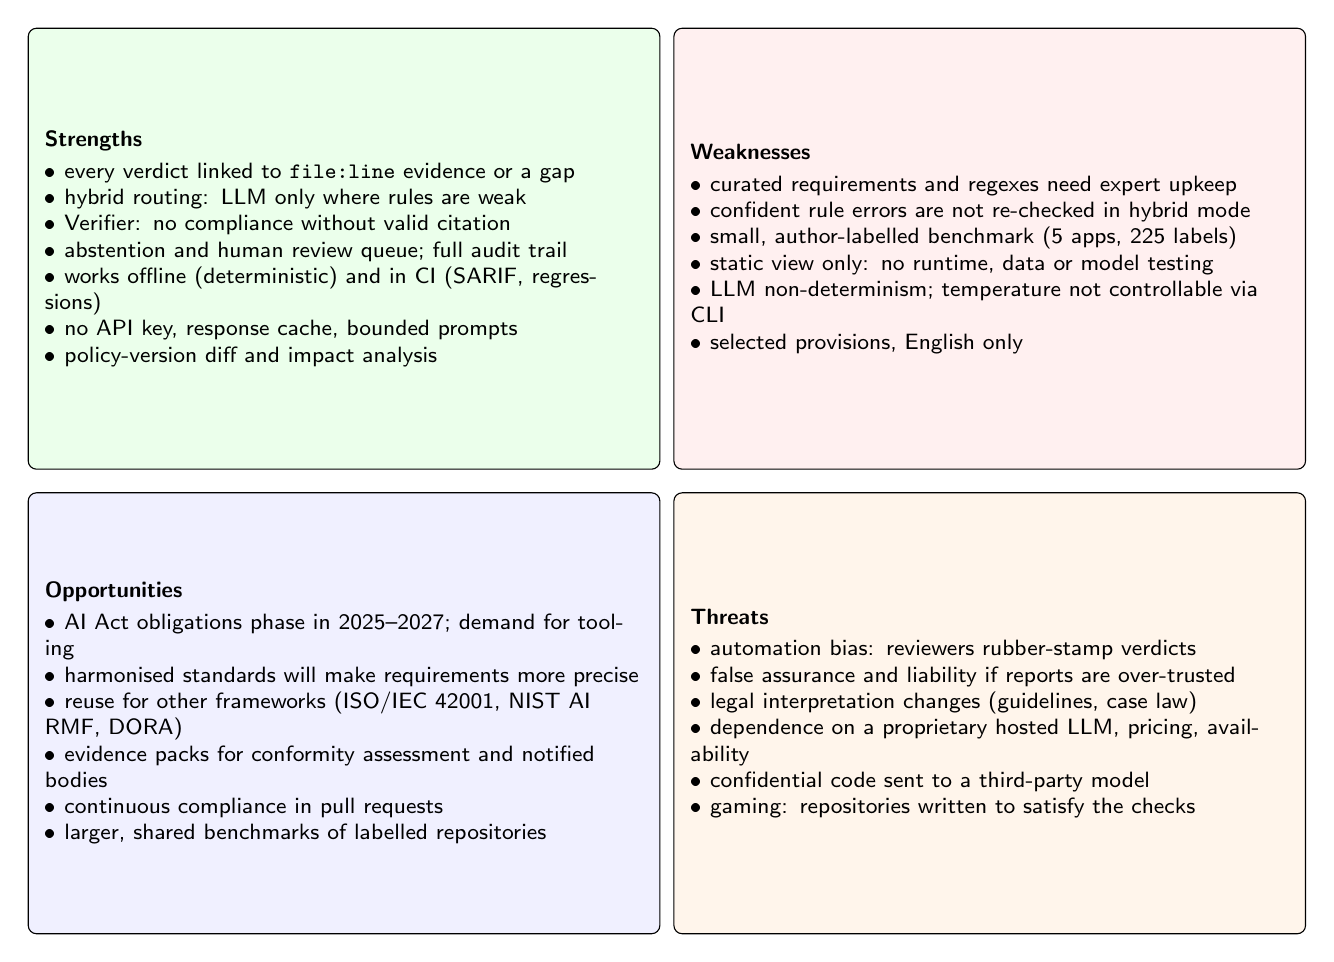
\begin{tikzpicture}[font=\sffamily\footnotesize,
  q/.style={draw, rounded corners=3pt, text width=7.6cm, minimum height=5.6cm, align=left, anchor=north west, inner sep=6pt}]
  \node[q, fill=green!8]  at (0,0)        {\textbf{Strengths}\\[2pt]
    \textbullet\ every verdict linked to \texttt{file:line} evidence or a gap\\
    \textbullet\ hybrid routing: LLM only where rules are weak\\
    \textbullet\ Verifier: no compliance without valid citation\\
    \textbullet\ abstention and human review queue; full audit trail\\
    \textbullet\ works offline (deterministic) and in CI (SARIF, regressions)\\
    \textbullet\ no API key, response cache, bounded prompts\\
    \textbullet\ policy-version diff and impact analysis};
  \node[q, fill=red!6]    at (8.2,0)      {\textbf{Weaknesses}\\[2pt]
    \textbullet\ curated requirements and regexes need expert upkeep\\
    \textbullet\ confident rule errors are not re-checked in hybrid mode\\
    \textbullet\ small, author-labelled benchmark (5 apps, 225 labels)\\
    \textbullet\ static view only: no runtime, data or model testing\\
    \textbullet\ LLM non-determinism; temperature not controllable via CLI\\
    \textbullet\ selected provisions, English only};
  \node[q, fill=blue!6]   at (0,-5.9)     {\textbf{Opportunities}\\[2pt]
    \textbullet\ AI Act obligations phase in 2025--2027; demand for tooling\\
    \textbullet\ harmonised standards will make requirements more precise\\
    \textbullet\ reuse for other frameworks (ISO/IEC 42001, NIST AI RMF, DORA)\\
    \textbullet\ evidence packs for conformity assessment and notified bodies\\
    \textbullet\ continuous compliance in pull requests\\
    \textbullet\ larger, shared benchmarks of labelled repositories};
  \node[q, fill=orange!8] at (8.2,-5.9)   {\textbf{Threats}\\[2pt]
    \textbullet\ automation bias: reviewers rubber-stamp verdicts\\
    \textbullet\ false assurance and liability if reports are over-trusted\\
    \textbullet\ legal interpretation changes (guidelines, case law)\\
    \textbullet\ dependence on a proprietary hosted LLM, pricing, availability\\
    \textbullet\ confidential code sent to a third-party model\\
    \textbullet\ gaming: repositories written to satisfy the checks};
\end{tikzpicture}
\caption{SWOT analysis of the Compliance-as-Code AI Auditor.}
\label{fig:swot}
\end{figure}

\paragraph{Mitigations.} Automation bias is countered by showing evidence before the verdict in the review sheet and by
requiring a justification for every override; vendor dependence by the backend protocol (any model behind
\texttt{complete\_json}) and the deterministic fallback; gaming by the LLM judge, which reads the whole context instead of
matching tokens, and by the decoy-style tests of the benchmark.
